\documentclass[5p,times]{elsarticle}
\usepackage{amsmath,amssymb,amsthm,mathtools,booktabs,graphicx,microtype}
\usepackage{tikz}
\usetikzlibrary{arrows.meta,patterns}
\usepackage[hidelinks]{hyperref}
\newtheorem{theorem}{Theorem}
\newtheorem{proposition}[theorem]{Proposition}
\newtheorem{lemma}[theorem]{Lemma}
\newtheorem{corollary}[theorem]{Corollary}
\theoremstyle{definition}\newtheorem{definition}[theorem]{Definition}
\theoremstyle{remark}\newtheorem{remark}[theorem]{Remark}
\newcommand{\R}{\mathbb R}\newcommand{\N}{\mathbb N}
\newcommand{\one}{\mathbf 1}\newcommand{\B}{\mathbf B}
\newcommand{\diag}{\operatorname{diag}}
\newcommand{\SOS}{\operatorname{SOS}}
\journal{Systems \& Control Letters}
\begin{document}
\begin{frontmatter}
\title{Beyond path-structured barrier certificates: exact embeddings, degree separation, and verified SOS synthesis}
\author[cub]{Reza Iraji\corref{cor1}}
\ead{reza.iraji@colorado.edu}
\author[cub]{Vishnu Murali}\ead{vishnu.murali@colorado.edu}
\author[cub]{Majid Zamani}\ead{majid.zamani@colorado.edu}
\cortext[cor1]{Corresponding author.}
\address[cub]{Department of Computer Science, University of Colorado Boulder, USA}
\begin{abstract}
Multiple-function safety certificates trade polynomial degree against the structure of the inequalities coupling their components. We characterize robust, globally scaled interpolation-inspired barrier certificates as anchored vector barrier certificates with weighted-path comparison matrices. The characterization specifies the direction of propagation, reciprocal weights, separation margins, and domain assumptions, and transports sum-of-squares witnesses without another optimization. To distinguish structural inclusion from genuine expressive power, we prove a finite-order obstruction: if a linear transition has finite order and no eigenvalue one, no implication-style interpolation-inspired certificate with affine frames exists, regardless of the number of frames. For explicit two- and four-dimensional rotation systems, cyclic affine vector certificates nevertheless prove safety, while quadratic scalar certificates also exist. The strict degree separation therefore holds before the scaled SOS relaxation is imposed. We implement polynomial synthesis in Julia and separate numerical candidate generation from exact-rational verification over invariant boxes. Reassessment of two polynomial examples identifies normalization and domain errors behind misleading feasibility comparisons. A source-matched external example, an explicitly labeled logistic-map adaptation, scalar baselines, and exact cyclic witnesses provide complementary reproducibility and structural tests. The resulting framework identifies both when certificate representations are interchangeable and when path structure genuinely increases the required degree.
\end{abstract}
\begin{keyword}
Safety verification \sep Vector barrier certificates \sep Interpolation-inspired certificates \sep Sum of squares \sep Exact verification
\end{keyword}
\end{frontmatter}

\section{Introduction}
Safety certificates separate initial states from unsafe states and establish that the separation is preserved along trajectories. A polynomial certificate can replace explicit reachable-set computation by a finite-dimensional search, but the choice of template remains consequential. A failure at a given polynomial degree can reflect the certificate conditions, the selected comparison parameters, an additional normalization, or numerical error. These causes should not be conflated.

Vector barrier certificates (VBCs) organize several scalar functions through an order-preserving comparison system. Their comparison-system foundation was developed for continuous dynamics by Sogokon et al.~\cite{sogokon}. Interpolation-inspired barrier certificates (IBCs) instead organize frame functions along a finite propagation sequence ending in a self-inductive frame~\cite{oumer}. The original implication-based IBC conditions and their globally scaled relaxations are different classes. This paper studies the latter under explicit full-domain and strict-separation assumptions; it does not identify every implication certificate with a matrix inequality.

The purpose of a relation between these constructions is operational rather than terminological. If two searches represent the same inequalities, an existing certificate and its algebraic proof should transfer between them without being rediscovered. Conversely, an apparent superiority of a general comparison matrix is meaningful only if it survives a matched template comparison. The mere fact that a matrix has additional nonzero entries proves neither a degree advantage nor the nonexistence of a different sparse comparison for the same functions.

We address both questions. First, we give an exact, bidirectional identification of globally scaled IBCs with a precisely anchored path-matrix VBC subclass. The identification includes the polynomial residuals used in synthesis, making it possible to transport SOS witnesses. Second, we prove a genuine fixed-degree separation. For a finite-order linear transition without eigenvalue one, every orbit has zero state average. An affine terminal frame has the same average on every orbit, and cannot have an invariant nonpositive sublevel set separating two nonempty orbit classes. This excludes affine implication-style IBCs independently of frame count and scaling choices. Cyclic affine VBCs escape the obstruction by permuting several components.

Graph-structured certificates are not new in themselves. In particular, path-complete barrier functions use graphs to express safety conditions for switched systems, and their completeness and ordering have been investigated by Anand et al.~\cite{anand}. Our result concerns an autonomous transition and the terminal invariant sublevel set required by an IBC. The exact representation theorem additionally assumes anchored, robust, globally scaled conditions. It is not a general ordering theorem for path-complete graphs. Likewise, numerical-to-rational SOS verification has established precedents~\cite{peyrl}; our contribution is its integration with exact certificate transport and a reproducible diagnosis of these specific representations.

The computational part has three purposes: to test the algebraic equivalence using transported proofs, to distinguish historical search failures from certificate nonexistence, and to expose the cost of path structure through an analytical benchmark with an exact impossibility proof. We use a source-matched BarrierBench entry~\cite{barrierbench,data}, a clearly identified autonomous adaptation of a logistic-map entry, and scalar baselines. The external examples test reproducibility, not superiority. The constructed finite-order examples establish the degree claim without relying on an infeasible SDP return.

\section{System and certificate classes}
Let
\begin{equation}\label{eq:system}
 x^+=f(x),\qquad x\in X\subset\R^n,
\end{equation}
where $f(X)\subseteq X$. The nonempty initial and unsafe sets $X_0,X_u\subseteq X$ are disjoint. Safety means $f^t(X_0)\cap X_u=\varnothing$ for every $t\in\N$, including $t=0$. All vector inequalities are componentwise. A comparison matrix $A\ge0$ is entrywise nonnegative, not merely positive semidefinite. In the polynomial experiments $X$ is a compact box with an independently established invariance proof.

Fix $\delta_0,\delta_u>0$. We distinguish robust separation from robust dynamics: the margins below do not imply safety under an unmodeled perturbation of $f$.
\begin{definition}[Anchored VBCs]\label{def:vbc}
A robust anchored forward VBC consists of $\B:X\to\R^m$ and $A\ge0$ satisfying
\begin{subequations}\label{eq:fv}
\begin{align}
 B_i(x)&\le-\delta_0 &&(x\in X_0,\ 1\le i\le m),\\
 B_1(x)&\ge\delta_u &&(x\in X_u),\\
 \B(f(x))&\le A\B(x) &&(x\in X).
\end{align}
\end{subequations}
A robust anchored backward VBC satisfies
\begin{subequations}\label{eq:bv}
\begin{align}
 B_i(x)&\le-\delta_u &&(x\in X_u,\ 1\le i\le m),\\
 B_1(x)&\ge\delta_0 &&(x\in X_0),\\
 \B(x)&\le A\B(f(x)) &&(x\in X).
\end{align}
\end{subequations}
The first component is the designated anchor; another fixed anchor can be moved there by a permutation.
\end{definition}
The anchor condition is stronger than requiring, for each unsafe state, some possibly state-dependent component to be positive. The exact correspondences below concern the anchored class. No necessity statement for polynomial certificates is inferred from set-theoretic indicator constructions.

\begin{proposition}[Soundness]\label{prop:sound}
Either certificate in Definition~\ref{def:vbc} proves safety of~\eqref{eq:system}.
\end{proposition}
\begin{proof}
For the forward condition, iteration gives $\B(f^t(x_0))\le A^t\B(x_0)\le0$, since $A^t\ge0$. The positive unsafe anchor excludes membership in $X_u$. For the backward condition, suppose $f^T(x_0)\in X_u$. Applying the backward inequality along that trajectory gives $\B(x_0)\le A^T\B(f^T(x_0))\le0$, contradicting the positive initial anchor. The case $T=0$ is covered by the separation conditions.
\end{proof}

\begin{definition}[Global scaled IBCs]\label{def:ibc}
Let $b_1,\ldots,b_m:X\to\R$ and $\lambda_1,\ldots,\lambda_m>0$. Write $s(i)=\min\{i+1,m\}$. A robust global scaled forward IBC satisfies
\begin{subequations}\label{eq:fi}
\begin{align}
 b_1(x)&\le-\delta_0 &&(x\in X_0),\\
 b_i(x)&\ge\delta_u &&(x\in X_u,\ 1\le i\le m),\\
 \lambda_i b_{s(i)}(f(x))&\le b_i(x) &&(x\in X,\ 1\le i\le m).
\end{align}
\end{subequations}
A robust global scaled backward IBC satisfies
\begin{subequations}\label{eq:bi}
\begin{align}
 b_1(x)&\le-\delta_u &&(x\in X_u),\\
 b_i(x)&\ge\delta_0 &&(x\in X_0,\ 1\le i\le m),\\
 b_{s(i)}(x)&\le\lambda_i b_i(f(x)) &&(x\in X,\ 1\le i\le m).
\end{align}
\end{subequations}
\end{definition}
These inequalities imply their corresponding nonpositivity implications. The converse need not hold. In particular, an implication restricted to $X\setminus X_u$ cannot be silently substituted for an all-$X$ comparison inequality. Requiring a uniform positive margin is also an explicit strengthening of weak separation. Neither strengthening is asserted to be without loss of generality.

\begin{definition}[Implication IBCs]\label{def:imp}
An implication-style forward IBC has $b_1\le0$ on $X_0$ and $b_i>0$ on $X_u$ for every $i$. Its propagation conditions are
\[
 b_i(x)\le0\ \Longrightarrow\ b_{s(i)}(f(x))\le0,
 \qquad x\in X\setminus X_u.
\]
An implication-style backward IBC has $b_1\le0$ on $X_u$, $b_i>0$ on $X_0$ for every $i$, and
\[
 b_i(f(x))\le0\ \Longrightarrow\ b_{s(i)}(x)\le0,
 \qquad x\in X.
\]
Here $s(i)=\min\{i+1,m\}$ includes the terminal self-loop. No uniform separation margin or global scaled inequality is required.
\end{definition}

\section{Exact representation and proof transport}
For $a_i>0$, define the weighted-path matrix $P(a)$ by
\begin{equation}\label{eq:path}
 P(a)_{i,s(i)}=a_i,\qquad P(a)_{ij}=0\ \text{otherwise}.
\end{equation}
For $m=1$, this is simply $[a_1]$. The row convention in~\eqref{eq:path} is fixed throughout; a drawing of directed edges is not used to determine indices.

\begin{theorem}[Exact global-scaled correspondence]\label{thm:embedding}
With the same functions, domains, and margins, sign reversal $\B=-b$ gives the equivalences
\begin{align*}
 \text{backward IBC with }\lambda
 &\ \Longleftrightarrow\ \text{forward VBC with }P(\lambda^{-1}),\\
 \text{forward IBC with }\lambda
 &\ \Longleftrightarrow\ \text{backward VBC with }P(\lambda),
\end{align*}
where the reciprocals are componentwise. Both directions preserve polynomial degree and the number of functions.
\end{theorem}
\begin{proof}
For~\eqref{eq:bi}, $b_{s(i)}\le\lambda_i b_i\circ f$ is equivalent, because $\lambda_i>0$, to
\[
 B_i\circ f\le\lambda_i^{-1}B_{s(i)}.
\]
This is exactly row $i$ of the forward comparison condition, including $i=m$. The initial inequalities become $B_i\le-\delta_0$ and the first unsafe inequality becomes $B_1\ge\delta_u$. These are~\eqref{eq:fv}. Every step is reversible.

For~\eqref{eq:fi}, $\lambda_i b_{s(i)}\circ f\le b_i$ becomes $B_i\le\lambda_i B_{s(i)}\circ f$. Its separation conditions become~\eqref{eq:bv}. This establishes the second equivalence and its converse. Sign reversal does not change degrees or dimensions.
\end{proof}

The theorem identifies a matrix representation, not every comparison inequality that a given function vector might satisfy. A vector admitted by a dense $A$ could also admit a path comparison. Matrix-support differences alone cannot exclude that possibility; Section~\ref{sec:separation} instead proves a template-level separation.

\begin{proposition}[Transport of SOS witnesses]\label{prop:transport}
Suppose each polynomial residual of a global scaled IBC has a representation
\begin{equation}\label{eq:representation}
 r=\rho+\sum_{j=0}^s g_j z_j^\top Q_j z_j+e,
 \quad Q_j\succeq0,\quad g_0=1,
\end{equation}
on its assigned domain, with $g_j\ge0$ there and a proved bound $|e|\le\beta\le\rho$. Its associated VBC in Theorem~\ref{thm:embedding} has a valid representation without solving a new SDP.
\end{proposition}
\begin{proof}
For a backward IBC, the propagation residual is
\[
 r_i=\lambda_i b_i\circ f-b_{s(i)}.
\]
The forward VBC residual is $r_i/\lambda_i$. Divide every $Q_j$, $\rho$, and $e$ by $\lambda_i$; positive semidefiniteness and $\beta/\lambda_i\le\rho/\lambda_i$ are preserved. For a forward IBC, the backward VBC residual is the identical polynomial $b_i-\lambda_i b_{s(i)}\circ f$. The separation residuals in both correspondences are unchanged and only need reordering. Thus all proofs transport with the certificate.
\end{proof}

This proposition provides a direct implementation test: coefficient identities must match before any optimization is attempted. Independent optimization is then optional. A comparison between a two-component VBC and a three-frame IBC, or between unrelated matrices, is not an experiment testing Theorem~\ref{thm:embedding}.

\begin{proposition}[Positive scaling and canonical path weights]\label{prop:scaling}
Let $D=\diag(d_1,\ldots,d_m)$ with $d_i>0$. The transformation
\[
 \widetilde\B=D\B,\qquad \widetilde A=DAD^{-1}
\]
preserves the appropriate forward or backward comparison inequality and strict component signs. For $A=P(a)$, take $d_1=1$ and $d_{i+1}=d_i a_i$. Then
\[
 \widetilde A=P(1,\ldots,1,a_m).
\]
\end{proposition}
\begin{proof}
The positive diagonal matrix $D$ preserves order. Substitution gives the comparison inequality in either direction. The transformed path entry is $d_i a_i/d_{i+1}=1$, while the terminal diagonal entry is $a_m$.
\end{proof}
Consequently, without fixed coefficient bounds or prescribed numerical margins, all transient path weights are redundant feasibility parameters. This elementary diagonal-similarity fact is not claimed as a new matrix theorem. Its synthesis consequence must be used carefully: margins scale componentwise, and a fixed coefficient budget is generally not invariant under $D$. A raw optimal margin from two differently normalized problems need not agree. Sign reversal, unlike arbitrary $D$, preserves a symmetric coefficient norm exactly.

\section{A strict degree separation}\label{sec:separation}
The next result distinguishes failure of a template class from failure of a numerical search.
\begin{lemma}[Finite-order scalar obstruction]\label{lem:finite}
Suppose $f^r=\mathrm{id}$ on $X$ for an integer $r\ge1$. If a real-valued $p$ takes both signs on $X$ and satisfies either
\[
 p\circ f\le a p\quad\text{or}\quad p\le a p\circ f,
 \qquad a>0,
\]
then $a=1$ and $p\circ f=p$ on $X$.
\end{lemma}
\begin{proof}
In the first case, iteration yields $p\le a^r p$. A positive value forces $a\ge1$, while a negative value forces $a\le1$. In the second case, iteration yields the same inequality $p\le a^r p$, with the same conclusion. When $a=1$, every finite orbit is a cycle of one-sided inequalities ending at its starting value. All inequalities on the cycle must therefore be equalities.
\end{proof}

\begin{theorem}[No affine implication IBC]\label{thm:obstruction}
Let $f(x)=Rx$, where $R^r=I$ and $1$ is not an eigenvalue of $R$. Let $R(X)=X$ and let $X_0,X_u\subset X$ be nonempty. No forward or backward implication IBC with affine frames exists, for any finite frame count. Consequently no robust global scaled affine IBC exists either.
\end{theorem}
\begin{proof}
In a forward implication IBC, propagating from $x_0\in X_0$ gives $b_m(R^{m-1}x_0)\le0$. At each preceding step the active frame is nonpositive, hence the state is not unsafe and the next implication applies. Write $p=b_m$ and $S=\{x\in X:p(x)\le0\}$. Then $S$ is nonempty and disjoint from $X_u$. The terminal implication gives $RS\subseteq S$. Since $R^r=I$, this implies $RS=S$.

In a backward implication IBC, propagating from $u\in X_u$ at successive preimages gives $b_m(R^{-(m-1)}u)\le0$. Now $S$ is nonempty and disjoint from $X_0$, and the terminal implication gives $R^{-1}S\subseteq S$. Finite order again implies $RS=S$.

In both cases, one orbit lies entirely in $S$, where $p\le0$, and another lies entirely in $X\setminus S$, where $p>0$. On the other hand,
\[
 (I-R)\sum_{j=0}^{r-1}R^j=I-R^r=0,
 \qquad \sum_{j=0}^{r-1}R^j=0,
\]
where the second equality uses invertibility of $I-R$. For the affine function $p(x)=c^\top x+d$, every orbit therefore has the same average:
\[
 \frac1r\sum_{j=0}^{r-1}p(R^jx)=d.
\]
The first orbit forces $d\le0$ and the second forces $d>0$, a contradiction. This argument does not require $X$ to have interior or the nonpositive value to be strictly negative. Global scaled certificates imply the corresponding sign implications, establishing the last assertion.
\end{proof}

\begin{corollary}[Tight affine--quadratic separation]\label{cor:rotation}
For $n=2$ or $4$, let $R$ be the block diagonal matrix with $n/2$ copies of
\[
 J=\begin{bmatrix}0&-1\\1&0\end{bmatrix}.
\]
Set $X=[-2,2]^n$. In $X_0$, every odd coordinate lies in $[0.9,1.1]$ and every even coordinate in $[-0.1,0.1]$. Let
\[
 X_u=[1.5,1.7]\times[-0.1,0.1]^{n-1}.
\]
An anchored forward VBC with $2n$ affine components exists. No implication IBC with affine frames exists, regardless of frame count. A quadratic scalar certificate, hence repeated quadratic IBC frames in both directions, does exist.
\end{corollary}
\begin{proof}
Take
\begin{equation}\label{eq:facets}
 \B(x)=(x_1-c,\ldots,x_n-c,-x_1-c,\ldots,-x_n-c)^\top,
 \quad c=6/5.
\end{equation}
The rotation permutes these components, so $\B(Rx)=A\B(x)$ for a permutation matrix $A\ge0$. On $X_0$ all components are at most $-1/10$, and on $X_u$ the first is at least $3/10$. This proves the VBC claim. Since $R^4=I$ and $1\notin\operatorname{spec}(R)$, Theorem~\ref{thm:obstruction} excludes every affine implication IBC.

Finally $g=x_1^2+x_2^2-3/2$ is invariant. On $X_0$, $g\le1.22-1.5=-0.28$, while on $X_u$, $g\ge2.25-1.5=0.75$. It is a quadratic scalar forward certificate. Repeating $g$ with unit scales gives a forward IBC; repeating $-g$ gives a backward IBC. Constant certificate vectors cannot separate the two nonempty sets, so the vector degree one and the IBC degree two are both minimal, for both implication and global scaled frames.
\end{proof}

\begin{figure}[t]
\centering
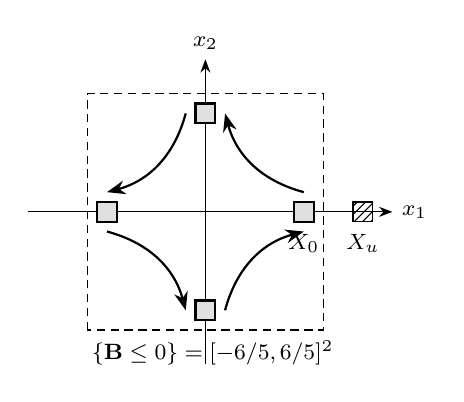
\begin{tikzpicture}[scale=1.25,>=Stealth,font=\footnotesize]
\draw[->] (-1.8,0)--(1.9,0) node[right]{$x_1$};
\draw[->] (0,-1.55)--(0,1.55) node[above]{$x_2$};
\draw[densely dashed] (-1.2,-1.2) rectangle (1.2,1.2);
\foreach \a in {0,90,180,270}{\begin{scope}[rotate=\a]
\draw[thick,fill=black!12] (.9,-.1) rectangle (1.1,.1);
\end{scope}}
\draw[->,thick] (1,.2) to[bend left=30] (.2,1);
\draw[->,thick] (-.2,1) to[bend left=30] (-1,.2);
\draw[->,thick] (-1,-.2) to[bend left=30] (-.2,-1);
\draw[->,thick] (.2,-1) to[bend left=30] (1,-.2);
\draw[pattern=north east lines] (1.5,-.1) rectangle (1.7,.1);
\node at (1.0,-.32) {$X_0$};\node at (1.6,-.32) {$X_u$};
\node[anchor=west] at (-1.25,-1.43) {$\{\B\le0\}=[-6/5,6/5]^2$};
\end{tikzpicture}
\caption{Exact two-dimensional structural example. The four initial-box images form a periodic orbit of sets. Cyclic comparison preserves four affine facets, whereas a terminal affine frame cannot separate the orbit classes. Arrows illustrate the discrete rotation, not continuous trajectories.}\label{fig:rotation}
\end{figure}

This is a polynomial-degree separation for both implication and global scaled IBCs, not a nonexistence claim for nonlinear frames or arbitrary scalar functions. The four-dimensional example is a block extension testing implementation generality, not a claim of high-dimensional computational scalability. The example is deliberately constructed; it is not represented as an external benchmark.

\begin{proposition}[Why a positive propagation reserve can be invalid]\label{prop:reserve}
For the cyclic construction above, there is no finite-valued $\B$ satisfying $\B(Rx)\le A\B(x)-\eta\one$ on $X$ with $\eta>0$ and its permutation matrix $A$.
\end{proposition}
\begin{proof}
Here $R^4=I$, $A^4=I$, and $A\one=\one$. Four iterations imply $\B(x)\le\B(x)-4\eta\one$, a contradiction.
\end{proof}
A numerical reserve is therefore a synthesis restriction, not part of the soundness theorem. Exact zero-residual propagation is essential for this example. The implementation supports zero reserve, and the structural witnesses are constructed exactly rather than inferred from a nearly feasible floating-point SDP.

\section{SOS synthesis and exact replay}
For a box $K=\prod_{j=1}^n[\ell_j,u_j]$ with $\ell_j<u_j$, use
\[
 g_j(x)=(x_j-\ell_j)(u_j-x_j)\ge0.
\]
Every separation or propagation obligation is written as a polynomial $p\ge0$ on its assigned box. For example, the forward VBC targets are $-B_i-\delta_0$, $B_1-\delta_u$, and $(A\B-\B\circ f)_i$. The forward IBC propagation target is $b_i-\lambda_i b_{s(i)}\circ f$, not its negative.

With a relaxation order $r$, numerical synthesis enforces
\begin{equation}\label{eq:sos}
 p=\rho+z_r^\top Q_0z_r+
 \sum_{j=1}^n g_j z_{r-1}^\top Q_jz_{r-1},\quad Q_j\succeq0,
\end{equation}
where $z_d$ lists monomials of total degree at most $d$. Coefficient matching is a polynomial identity, not collocation at sampled points. The order must satisfy $2r\ge\deg(p)$; in particular, composition can raise degree to $\deg(B_i)\deg(f)$. The implementation uses JuMP and SumOfSquares.jl with CSDP~\cite{sos,csdp}.

Each solve fixes $A$ or $\lambda$. Joint optimization with unknown certificate coefficients is bilinear and is not claimed to be an SDP. We use feasibility, not margin maximization: $\delta_0=\delta_u=10^{-3}$ for free synthesis, a per-component coefficient $\ell_1$ bound of one, and a declared reserve $\rho=10^{-6}$. This normalization is closed under sign reversal. These bounds are experiment settings, not necessary conditions for safety.

A solver return alone is insufficient for acceptance. Coefficients and Gram matrices are converted to rational numbers, and the checker reconstructs every target from the versioned rational dynamics, sets, and certificate coefficients. It does not trust an exported target polynomial or a solver's boolean status. Positive semidefiniteness is checked by exact rational elimination, including zero pivots. If a small diagonal shift is used to obtain an exactly PSD matrix, its effect is included in the residual, never discarded.

\begin{theorem}[Residual-budget acceptance]\label{thm:replay}
Suppose rational $Q_j\succeq0$ define $s(x)=\sum_{j=0}^n g_j(x)z_j(x)^\top Q_jz_j(x)$ on $K$, with $g_0=1$. Write $e=p-\rho-s=\sum_\alpha e_\alpha x^\alpha$. Let $M_j=\max\{|\ell_j|,|u_j|\}$ and
\begin{equation}\label{eq:error}
 \beta=\sum_\alpha |e_\alpha|\prod_j M_j^{\alpha_j}.
\end{equation}
If $0\le\beta\le\rho$, then $p\ge0$ everywhere on $K$.
\end{theorem}
\begin{proof}
Each term in $s$ is nonnegative on $K$. The monomial bound gives $|e|\le\beta$. Thus $p=\rho+s+e\ge\rho-\beta\ge0$.
\end{proof}
The bound can be conservative; a failed replay is inconclusive, not proof of an invalid certificate. The checker uses exact rational arithmetic but is not a proof-assistant mechanization. This is a different acceptance route from demanding an exactly reconstructed SOS identity with zero residual, although both build on established numerical-symbolic certification principles~\cite{peyrl}.

Certificates, Gram matrices, margins, reserves, comparison parameters, solver status, and exact replay outcomes are serialized separately. Tests cover reciprocal weights, terminal loops, changed benchmark data, malformed or indefinite Gram matrices, serialization, and deliberately modified certificates. Every published acceptance also requires the registered verification domain to be invariant. Time measurements in the audit are explicitly optimizer-call timings and are not used to claim end-to-end speedups.

\section{Diagnostic and external examples}\label{sec:experiments}
The suite separates four questions: correctness of existing examples, source-matched reproduction, an explicitly changed nonlinear task, and a strict template obstruction. This separation avoids presenting easy external examples as evidence of an expressive advantage or presenting a constructed example as an established application benchmark.

\subsection{Two polynomial diagnostic systems}
The first system is
\begin{align*}
 f_1(x)&=0.72x_1+0.10x_2-0.12x_1^3,\\
 f_2(x)&=-0.08x_1+0.68x_2-0.08x_2^3,
\end{align*}
with $X=[-1.4,1.4]^2$, $X_0=[-0.2,0.2]^2$, and $X_u=[0.95,1.25]^2$. Write $f(x)=M(x)x$. Its diagonal entries are nonnegative on $X$; absolute row and column sums give $\|M(x)\|_\infty\le0.82$ and $\|M(x)\|_1\le0.80$. Hence, for $V=x_1^2+x_2^2$,
\[
 V(f(x))\le(82/125)V(x).
\]
The explicit polynomials $g=V-1/10$ and $h=-g$ satisfy
\begin{align*}
 (4/5)g-g\circ f&\ge(18/125)V+1/50,\\
 (6/5)h\circ f-h&\ge(133/625)V+1/50.
\end{align*}
Moreover $g\le-1/50$ on $X_0$ and $g\ge341/200$ on $X_u$. Exact SOS witnesses for all four formulations are included in the artifact. Thus absence of backward quadratic certificates is not an explanation for a failed search on this example.

A former coefficient restriction, $c_{x_1^2}+c_{x_2^2}=1$ with both coefficients positive, excludes $h$ and is not closed under sign reversal. The controlled normalization ablation reinstates that restriction while keeping the other new SOS settings fixed. Its reported infeasibility is a solver outcome for that restriction, not an exact nonexistence theorem. Since $X_0$ itself is invariant, this system is a correctness check rather than a demanding reachability task.

The second system is
\begin{align*}
 f_1(x)&=1.05x_1+0.18x_2-0.10x_1^3,\\
 f_2(x)&=0.02x_1+0.92x_2,
\end{align*}
with $X_0=[-0.12,0.12]^2$ and $X_u=[0.85,1.10]\times[-0.10,0.10]$. The original box $[-1.4,1.4]\times[-1.2,1.2]$ is not invariant. At its corner, $f_1(1.4,1.2)=1.4116$. We instead use $X=[-1.5,1.5]\times[-1.2,1.2]$, retaining the same dynamics and safety sets. Positive coordinate derivatives and odd symmetry establish exact absolute image bounds $1.4535$ and $1.134$. Unlike the first system, its initial box is not invariant: $f_1(0.12,0.12)=0.1474272>0.12$.

The historical grid-based implementation and result files are retained as labeled legacy material. They are not represented as earlier SOS proofs or used in the new comparison table.

\subsection{External provenance and nonlinear adaptation}
BarrierBench is a recent collection covering both controlled and autonomous, continuous- and discrete-time problems~\cite{barrierbench,data}. We reproduce the autonomous entry whose transition simplifies exactly to
\[
 f(x)=(-x_2/100,\ x_1/100),
\]
with $X_0=[0.1,0.4]\times[0.1,0.55]$ and $X_u=[0.45,0.5]\times[0.6,1]$. We add the invariant verification box $[-1.2,1.2]^2$, without changing the transition or either safety set. It is a contraction; its initial states leave the initial box after one step.

The second external-data-derived task uses
\[
 f_1(x)=\tfrac{16}{5}x_1(1-x_1),\qquad
 f_2(x)=\tfrac{14}{5}x_2(1-x_2),
\]
with $X=[0,1]^2$, $X_0=[0.1,0.3]\times[0.2,0.4]$, and $X_u=[0.8,1]^2$. The logistic family is classical~\cite{may}. The cited dataset entry is controlled; here both inputs are fixed to zero. We therefore label this case \emph{Logistic-adapted}, not an exact reproduction of the original controller-synthesis problem, and do not import the dataset's supplied controller or barrier as evidence. The map has image in $[0,0.8]\times[0,0.7]$, proving domain invariance. This is a nonlinear verification test, not a claimed chaotic benchmark.

Widely used continuous-time and hybrid reachability collections such as ARCH-COMP~\cite{arch} serve a different semantic setting. Replacing an ODE with an Euler step does not preserve its safety problem without an approximation-error argument. We therefore do not report results on such a surrogate as verification of the original ODE benchmark.

\subsection{Matched protocol and reported outcomes}
The four free-synthesis problems use three components or frames and degree two. Their forward VBC path weights are respectively $4/5$, $17/20$, $4/5$, and $1/10$; backward VBC path weights are $6/5$, $6/5$, $6/5$, and $10$. IBC scales are obtained by the exact mapping in Theorem~\ref{thm:embedding}. Relaxation orders are three for the cubic systems and two for the two external-data cases. Scalar forward baselines use the same forward gain and degree, with order three. The repeated-facet rotation certificates are exact analytical witnesses with zero propagation reserve, not outcomes of free SDP searches.

\begin{table}[t]
\centering\small
\caption{Recorded exact-replay outcomes. V denotes an accepted exact-rational proof, not merely a feasible solver status. Any other outcome is retained as an explicit status. The scalar column is a forward degree-two baseline.}\label{tab:results}
\begin{tabular}{lccccc}\toprule
Problem & fVBC & bVBC & fIBC & bIBC & Scalar\\\midrule
S1 & V & V & V & V & V\\
S2 (repaired) & V & V & V & V & V\\
BB rotation & V & V & V & V & V\\
Logistic-adapted & V & V & V & V & V\\
\bottomrule\end{tabular}
\end{table}

For each accepted IBC solution, the existing Gram witnesses are transported to the corresponding VBC and replayed without re-optimization. These checks test the claimed representation directly. They do not establish equality of independently optimized margins under arbitrary rescaling. All sixteen multi-function searches and all four scalar forward baselines passed exact-rational replay. Consequently, these four examples do not establish a multiple-function advantage. The controlled legacy-normalization ablation returned no certified candidate, a solver outcome rather than an exact nonexistence theorem.

The rotation systems have no affine implication IBC for any finite frame count, while their cyclic witnesses replay with zero residual. The four-dimensional block extension does not establish scalability, and no ranking against tools with different semantics is inferred.

\section{Conclusion}
Global scaled IBCs have an exact anchored path-matrix interpretation, provided direction, reciprocal weights, strict separation, and propagation domains are aligned. This interpretation transports both certificates and their SOS proofs. General matrix support is not itself evidence of expressive power; a finite-order obstruction instead proves a strict affine--quadratic separation between cyclic VBCs and implication-style IBCs of arbitrary finite length. Periodicity also shows why a strictly positive propagation reserve can create artificial infeasibility. A Julia implementation separates numerical synthesis from exact-rational replay and makes normalization, domain repair, provenance, and scalar baselines explicit. These results distinguish representation, template nonexistence, and numerical uncertainty.

\section*{Reproducibility and data availability}
The accompanying artifact contains Julia source, a resolved package manifest, benchmark definitions, proof files, replay scripts, tests, and the recorded results. Numerical data are bound to the tested source revision and checksums in the evidence directory. A private development repository is not presumed accessible to reviewers; the same source and evidence should accompany the submission as an artifact. No benchmark-data or code license is inferred beyond the cited source terms.

\section*{Acknowledgments}
This work is supported partially by NSF grants CNS-2039062 and CNS-2111688.

\section*{Declaration of generative AI use}
ChatGPT was used to assist with literature searches, code development, mathematical drafting, and preparation of the initial manuscript. Responsibility for verification, interpretation, and the final submitted text rests with the authors.

\bibliographystyle{elsarticle-num}
\bibliography{references}
\end{document}
